% --- Medical-domain application: MedSAM (foundation model for medical image segmentation) ---
\begin{frame}{Medical Application: MedSAM --- Segment Anything in Medicine}
  \begin{columns}[T,onlytextwidth]
    \begin{column}{0.56\textwidth}
      \textbf{The problem}
      \begin{itemize}\itemsep0.22em
        \item Clinical segmentation (tumours, organs, lesions) is usually \textbf{narrow}:
              one model per modality, organ, and task.
        \item Expert pixel-level labels are scarce and expensive.
      \end{itemize}
      \vspace{0.4em}
      \textbf{The foundation-model answer}
      \begin{itemize}\itemsep0.22em
        \item \textbf{MedSAM} adapts the \textbf{Segment Anything Model (SAM)} to medicine by
              fine-tuning on $>$1M medical image--mask pairs.
        \item Spans \textbf{10+ imaging modalities} (CT, MRI, X-ray, ultrasound, pathology,
              endoscopy) and \textbf{30+ cancer types}.
        \item \textbf{Promptable:} a clinician gives a bounding box; the model returns the mask
              --- one model generalising across tasks.
      \end{itemize}
    \end{column}
    \begin{column}{0.44\textwidth}
      \textbf{Why it matters here}
      \begin{itemize}\itemsep0.22em
        \item A concrete case of the \textbf{pretrain-once, adapt-widely} paradigm reaching a
              high-stakes domain.
        \item Same recipe as the vision FMs earlier in this lecture (SAM, CLIP), now
              \textbf{domain-specialised} via large-scale fine-tuning.
        \item Complements \textbf{TRIBE\,v2} (brain-response modelling): together they show
              foundation models spanning \textbf{imaging} and \textbf{physiological} medical data.
      \end{itemize}
      \vspace{0.5em}
      {\footnotesize Ma et al., ``Segment Anything in Medical Images'' (MedSAM),
      \emph{Nature Communications} 2024
      (\href{https://www.nature.com/articles/s41467-024-44824-z}{doi:10.1038/s41467-024-44824-z};
      \href{https://arxiv.org/abs/2304.12306}{arXiv:2304.12306}).}
    \end{column}
  \end{columns}
\end{frame}

\begin{frame}{MedSAM: Architecture}
  \centering
  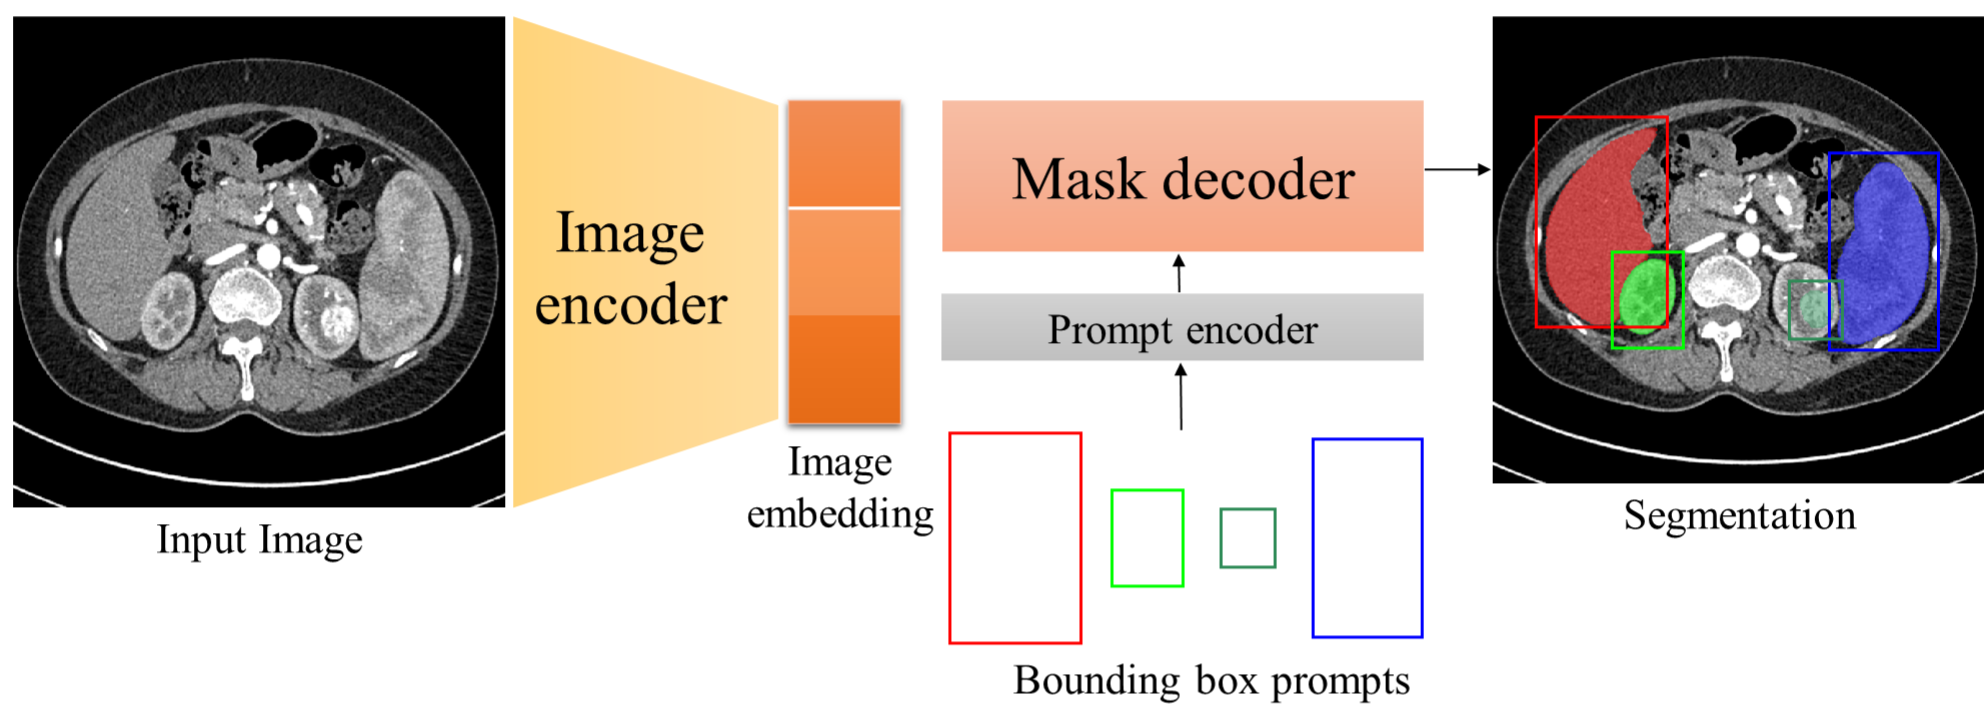
\includegraphics[width=\linewidth,height=0.84\textheight,keepaspectratio]{images/med-sam/MedSAM_architecture.png}\\[0.2em]
  {\scriptsize An image encoder and prompt encoder feed a mask decoder; only the box prompt is used at
  inference. Source: Ma et al., MedSAM (\href{https://arxiv.org/abs/2304.12306}{arXiv:2304.12306}).}
\end{frame}

\begin{frame}{MedSAM: Segmentation across modalities}
  \centering
  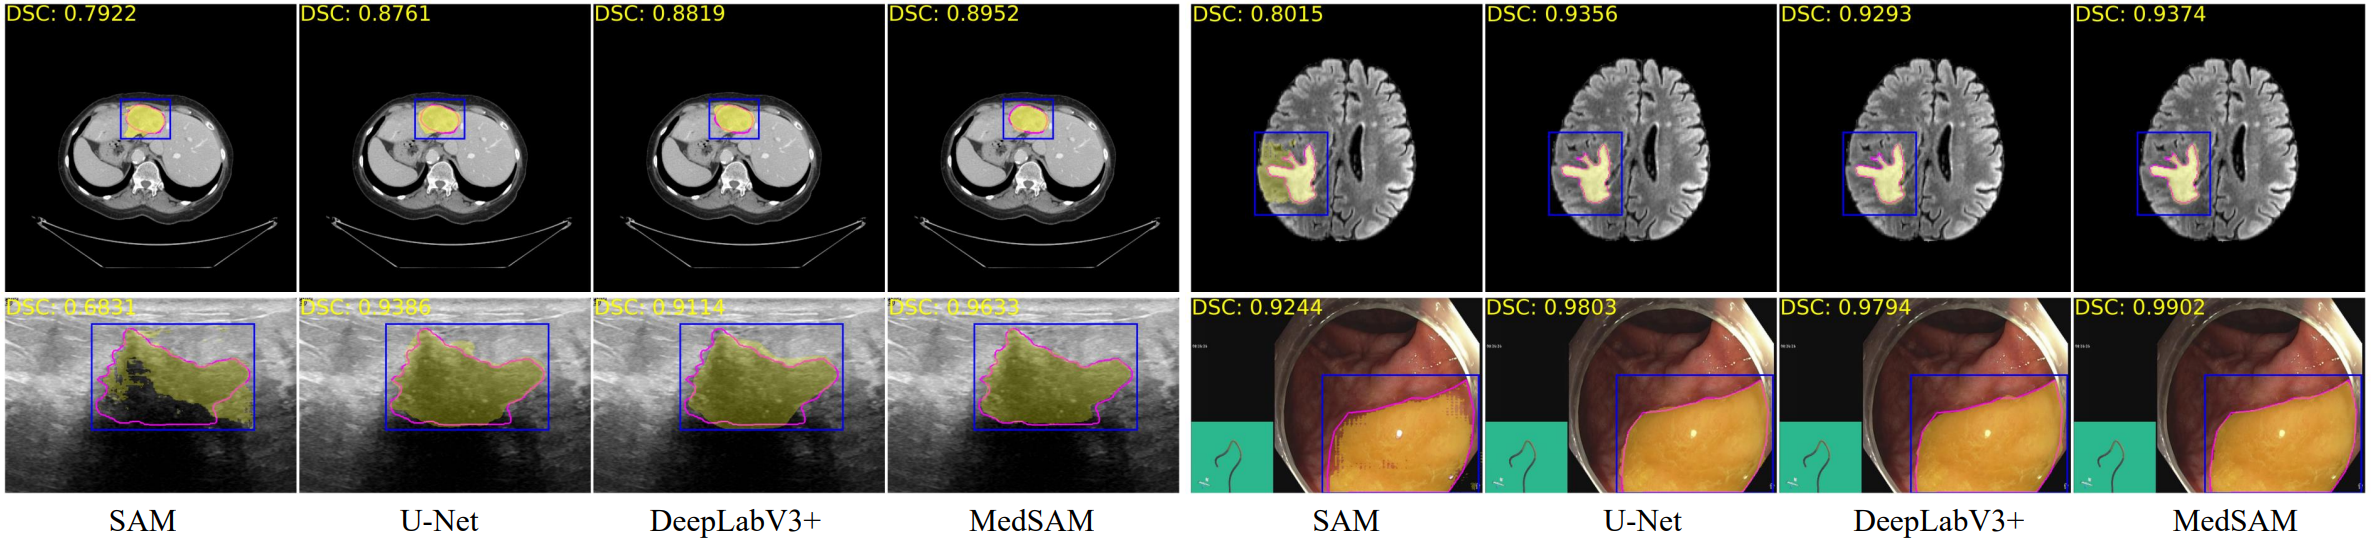
\includegraphics[width=\linewidth,height=0.84\textheight,keepaspectratio]{images/med-sam/MedSAM_examples.png}\\[0.2em]
  {\scriptsize One promptable model segments targets across CT, MRI, ultrasound, pathology, and more.
  Source: Ma et al., MedSAM (\href{https://arxiv.org/abs/2304.12306}{arXiv:2304.12306}).}
\end{frame}
